A evolução dos sistemas de comunicações sem fio, fomentou a implementação de diversas aplicações móveis. Neste contexto, melhorar a eficiência energética desses sistemas se torna uma característica desejável, tanto para os dispositivos móveis que buscam melhorar a autonomia das baterias quando para os sistemas de comunicação radio base que, tendem a perder energia em forma de calor.  
Sendo assim, o sistema de comunicação pode ser dividido em 3 sub-sistemas principais: Meio transmissor, Receptor e o Transmissor, conforme argumentado por \cite{Schuartz2017}.
No entanto, este trabalho foca exclusivamente no sistema transmissor, ilustrado pela figura \ref{fig:sistemadetrasmissao}, em que observa-se diversos componentes que compõem o transmissor de sinal entre esses elementos o amplificador de potência é o componente de maior demanda energética, por se tratar do componente que converte a energia da fonte em energia irradiada pela antena de transmissão. Portanto, a eficiência do sistema de transmissão depende diretamente do desempenho do transmissor. 

% // TODO Refazer figura
\begin{figure}[!ht!]
    \centering
    \captionsetup{justification=centering}
    \caption*{Fonte: \cite{Schuartz2017}}
    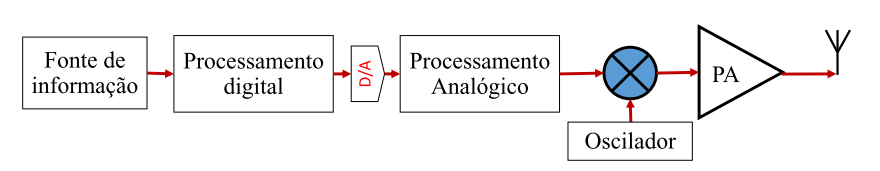
\includegraphics[width=0.5\textwidth]{sistematrasmissorpng.png}
    \caption{Sistema de transmissão simplificado}
    \label{fig:sistemadetrasmissao}
\end{figure}

Considerando também que a largura de banda reservada para sistemas de comunicação sem fio é reduzida, torna-se desejável que ela seja utilizada da maneira mais eficiente o possível. Diante desse cenário, segundo \cite{Kenington2000}, só é possível alcançar as maiores taxas utilizando estratégias de modulações, que alterem tanto a fase quanto a amplitude de uma onda portadora em rádio frequência. Ainda segundo \cite{Kenington2000}, a modulação na amplitude, exige linearidade na transmissão afim de evitar erros e interferência na comunicação entre os usuários vizinhos. Ante esse panorama, o projetista do PARF se depara com esse desafio, que é desenvolver um hardware eficiente energeticamente e com uma boa linearidade, o que é um compromisso é conflitante, conforme descrito por \cite{Cripps2006}. Esse comportamento se deve, ao fato que um PARF atua de forma eficiente, ou seja, com baixo consumo de energia, na área próxima à de saturação, que é a região em que opera em regimes não lineares, conforme ilustrado pela figura \ref{fig:saidaparf}.



\begin{figure}[ht!]
    \centering
    \captionsetup{justification=centering}
    \caption*{Fonte: \cite{Chavez2018}}
    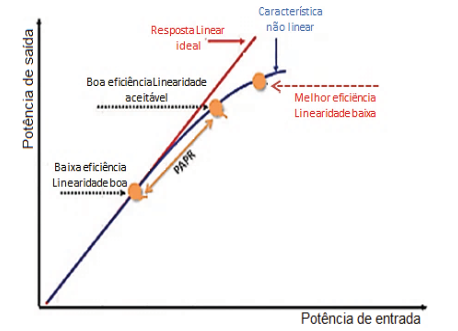
\includegraphics[width=0.5\textwidth]{curvasaidaparf.png}
    \caption{Curva de saída do amplificador}
    \label{fig:saidaparf}
\end{figure}

A fim de contornar esse obstáculo foi adicionado a cadeia de transmissão um método de equalização de sinais, conforme argumentado por \cite{Kenington2000}. Um exemplo de técnica de linearização de sinais é a implementação de um pré-distorcedor de sinais digitais em banda base, o qual apresenta um melhor custo-benefício \cite{Kenington2000}. Essa técnica consiste em distorcer o sinal de entrada utilizando técnicas de processamento digital, antes que esse module uma portadora, de forma compensativa à distorção causada pelo PARF. De maneira sucinta, o DPD é conectado em cascata ao PARF e é projetado de forma que apresenta a função transferência inversa ao PARF. Para isso, é necessário um modelo de alta precisão e baixa complexidade computacional, capaz de representar as características de transferência direta e inversa de um PARF. Isso significa modelar o seu comportamento real utilizando um software.  A figura \ref{fig:cascatadpd} ilustra o processo do um pré-distorcedor digital.

\begin{figure}[h!]
    \centering
    \captionsetup{justification=centering}
    \caption*{Fonte: \cite{Chavez2018}}
    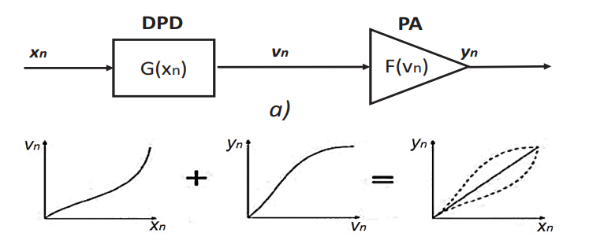
\includegraphics[width=0.5\textwidth]{DPDcascata.png}
    \caption{ilustração do pré-distorcedor em cascata}
    \label{fig:cascatadpd}
\end{figure}

Segundo \cite{John2016}, existem duas técnicas utilizadas para fazer essa modelagem. Uma consiste na descrição detalhada do PARF, que implica em uma maior complexibilidade computacional, esses modelos são conhecidos como modelos físicos. A outra abordagem é conhecida como modelo empírico, este modelo consiste em coletadas amostradas na entrada e na saída do PARF em domínio temporal, e através destes dados simulam um modelo matemático do sistema. Uma das vantagens desse método é que ele não exige conhecimento prévio da estrutura do PARF e possui baixa complexidade computacional e mesmo se todos os parâmetros fossem conhecidos o equacionamento completo do circuito, uma função inversa poderia ser encontrada, possivelmente muito mais complexa que séries de Volterra. No entanto, sua precisão pode ser ligeiramente afetada pelo modelo adotado. 
Sendo assim, como a proposta do projeto é a implementação de um DPD em hardware, se faz necessário que o circuito apresente a menor complexidade possível,  torna-se mais viável fazer a implementação utilizando modelagem matemática. 

\section{Modelagens Matemáticas}

\subsection*{Séries de Volterra}
Segundo \cite{Gonçalves2009} série de Volterra pode ser vista como uma extensão multidimensional da série de Taylor para sistemas dinâmicos. A modelagem começa com a representação do sistema através de uma série infinita de integrais convolucionais, em que cada termo da série corresponde a uma ordem de não linearidade e memória.

A saída \( y(t) \) de um sistema pode ser expressa pela equação \ref{eq:Volterra}: \begin{equation}
    y(t) = h_0 + \sum_{n=1}^{\infty} \int_{-\infty}^{\infty} \cdots \int_{-\infty}^{\infty} h_n(\tau_1, \tau_2, \ldots, \tau_n) \prod_{i=1}^{n} x(t - \tau_i) \, d\tau_i
    \label{eq:Volterra}
\end{equation} onde \( h_n \) são os núcleos de Volterra, que caracterizam a resposta do sistema para a \( n \)-ésima ordem de não linearidade e \( x(t) \) é a entrada do sistema.

Os núcleos de Volterra \( h_n \) são funções de várias variáveis que capturam a dinâmica do sistema em diferentes ordens. Para a maioria das aplicações práticas, a série é truncada para incluir apenas um número finito de termos, já que a identificação de todos os núcleos de uma série infinita é impraticável.

\subsection*{Polinômio de memória}\label{sub:polimem}

Um modelo simples, utilizado na modelagem comportamental simplifificada das séries de Volterra considerando apenas componentes unidimensionais\footnote{Cada termo do somatório é composto por amostras no mesmo instante, por exemplo: $x(n)|x(n)|,x(n - 1)|x(n - 1)|$; termos bidimensionais são compostos por amostras em instantes de tempos distintos, como por exemplo: $x(n)|x(n - 1)|$} é o MP, que é um modelo compacto, de baixo custo computacional e linear em seus parâmetros. O MP gera baixo erro quando aplicado à PAs que apresentam pouco efeito de memória. O DPD e pós distorsor apresentam uma característica de transferência inversa a do PA \cite{Schuartz2017}, portanto o mesmo modelo pode ser utilizado. A equação \ref{eq:mp} apresenta o MP conforme apresenta \cite{Schuartz2017}: 

\begin{equation}
    y(n) = \sum_{p=1}^{P} \sum_{m=0}^{M} h_{p,m} x(n - m) \left| x(n - m) \right|^{p-1}
    \label{eq:mp}
\end{equation}

Como a proposta do trabalho é a implementação em hardware desse modelo, torna-se necessário paralelizar operações aritméticas de forma a alcançar uma taxa de operação que satisfaça a norma regulamentadora. Nesse contexto, as FPGAs apresentam-se como uma alternativa viável para a implementação de circuitos pré-distorcedores 

\section{FPGAs}

Como descrito em \cite{Pedroni2010}, FPGAs são uma classe de dispositivos lógicos programáveis que permitem a reconfiguração física de seus componentes de eletrônica digital por meio de uma linguagem de descrição de hardware. Basicamente, as FPGAs consistem em um conjunto de subcircuitos digitais interconectados, capazes de realizar diversas funções comuns enquanto oferecem um alto nível de flexibilidade. Devido a essas características, FPGAs podem ser utilizadas para aplicações como processamento de imagem em tempo real e aprendizado de máquina.

FPGAs têm a capacidade de sintetizar arquiteturas complexas de eletrônica digital, resultando em um funcionamento altamente paralelizado que permite um processamento rápido com várias portas de entrada e saída. Além disso, elas também suportam o desenvolvimento de códigos sequenciais.

A estrutura interna de uma FPGA é composta fundamentalmente por blocos lógicos interligados, organizados em uma matriz. Cada bloco é formado por diversos sub-blocos, que por sua vez contêm os componentes mais básicos da hierarquia. FPGAs da Intel e da Xilinx possuem nomenclaturas e organizações diferentes para esses blocos e sub-blocos. Isso é ilustrado na Figura \ref{fig:Stratix} e na Figura \ref{fig:Ultrascale}, que mostram as FPGAs Intel Stratix X e Xilinx Ultrascale+, respectivamente. Embora as arquiteturas sejam fundamentalmente semelhantes, com a disposição em matriz dos blocos e funcionalidades dos componentes fundamentais sendo universais, os blocos lógicos são denominados LAB nas FPGAs da Intel e CLB nas FPGAs da Xilinx. Os sub-blocos são chamados de ALM ou LE, dependendo da FPGA da Intel, e de Slices nas FPGAs da Xilinx.

\begin{figure}[h!]
    \centering
    \captionsetup{justification=centering}
    \caption*{Fonte: \cite{Pedroni2010}}
    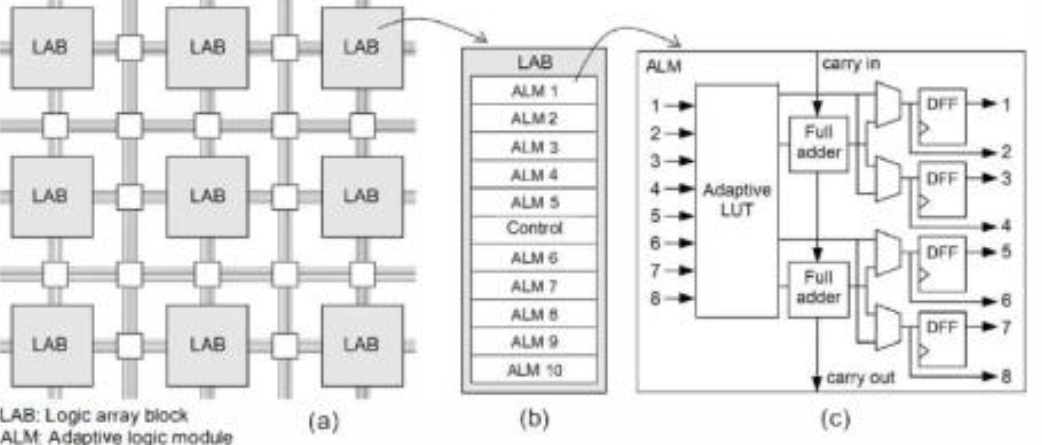
\includegraphics[width=0.75\textwidth]{FPGA Stratix X da Intel.png}
    \caption{Estrutura Interna da FPGA Stratix X da Intel}
    \label{fig:Stratix}
\end{figure}

\begin{figure}[h!]
    \centering
    \captionsetup{justification=centering}
    \caption*{Fonte: \cite{Pedroni2010}}
    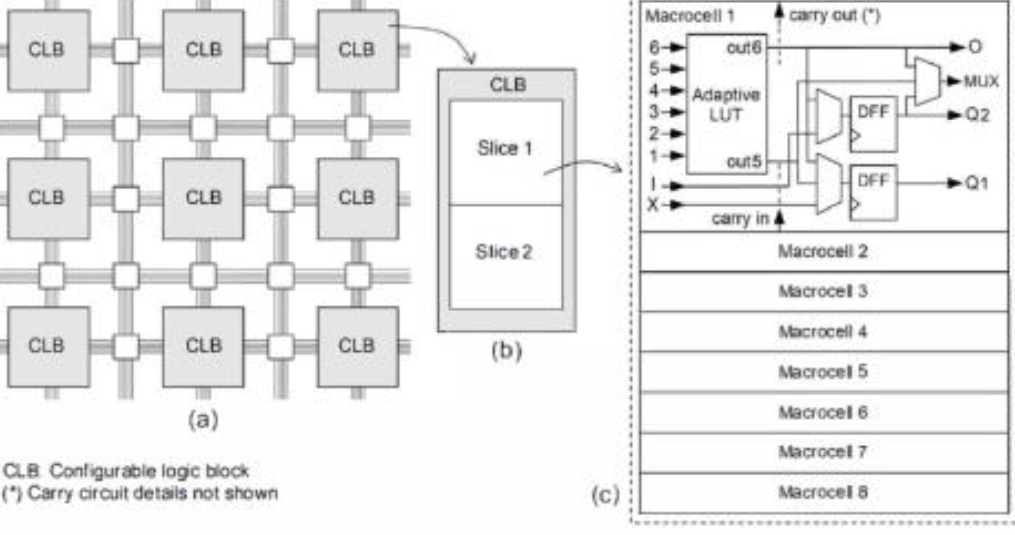
\includegraphics[width=0.75\textwidth]{FPGA Ultrascale+.png}
    \caption{Estrutura Interna da FPGA Ultrascale+}
    \label{fig:Ultrascale}
\end{figure}

Os sub-blocos das FPGAs são compostos por LUTs e registradores. As LUTs são compostas por uma árvore binária de multiplexadores 2:1, permitindo o armazenamento de uma função lógica na forma de SOP. Os registradores são os componentes síncronos dos sub-blocos. Além da estrutura mencionada, FPGAs comumente possuem diversos módulos integrados, como CPUs, DSPs, memória Flash, PLLs, que aumentam ainda mais as capacidades do FPGA.

As FPGAs são programadas utilizando uma linguagem de descrição de hardware, sendo o VHDL uma das mais comuns para a síntese de circuitos integrados de alta velocidade. Criada por uma iniciativa financiada pelo Departamento de Defesa dos Estados Unidos em meados dos anos 80, o VHDL foi a primeira linguagem de descrição de hardware padronizada pela IEEE.

A estrutura de um código VHDL consiste em três partes principais: declaração de bibliotecas/pacotes, entidade e arquitetura. Na primeira parte, são listadas as bibliotecas e pacotes necessários para o projeto. As bibliotecas padrão incluem a `std` e a `work`. A entidade, que é a interface do sistema, descreve as entradas e saídas e é dividida em duas partes: parâmetros e conexões. Os parâmetros são valores constantes, como a largura de um barramento, que são declarados como genéricos. As conexões, por sua vez, definem a transferência de informações e correspondem aos pinos de entrada e saída do circuito. Já a arquitetura é a parte principal do sistema, na qual o circuito é descrito. Nessa seção, são definidas as atribuições, operações lógicas e aritméticas, comparações, entre outros. Há também uma parte declarativa da sintaxe, que apresenta uma ampla variedade de declarações possíveis.

Dessa forma, circuitos digitais para processamento de sinais em tempo real são muito utilizados em sistemas de comunicações sem fio. Um exemplo de aplicação são os DPDs para transmissores sem fio. Os DPDs são baseados em operações matemáticas que envolvem uma grande quantidade de somas, produtos e tabelas de busca. Devido às rigorosas exigências de frequência de operação, torna-se fundamental a paralelização das operações necessárias. Nesse contexto, as FPGAs se mostram uma alternativa viável para a implementação de circuitos DPDs, especialmente devido à sua capacidade de paralelização. Considerando que a paralelização em FPGAs pode alcançar uma taxa de operação adequada para o uso pretendido, a implementação desse hardware em um circuito lógico dedicado pode oferecer resultados ainda mais eficientes para essa aplicação, dado o potencial de otimização específica e o desempenho superior de circuitos dedicados em relação a arquiteturas reconfiguráveis.

\section{Síntese com as células da tecnologia}
A concepção o circuito lógico do DPD segue o fluxo de projeto VLSI para design de um circuito integrado de aplicação específica, inclui a descrição do circuito em VHDL, síntese lógica utilizando as células padrão da tecnologia, PAR (\textit{place and route}) e simulações comportamentais e temporais. O diagrama do fluxo VLSI pode ser ilustrado pela figura \ref{fig:CMOS2010}.

\begin{figure}[ht!]
	\centering
	\captionsetup{justification=centering}
	\caption*{Fonte: \cite{CMOS2010}}
	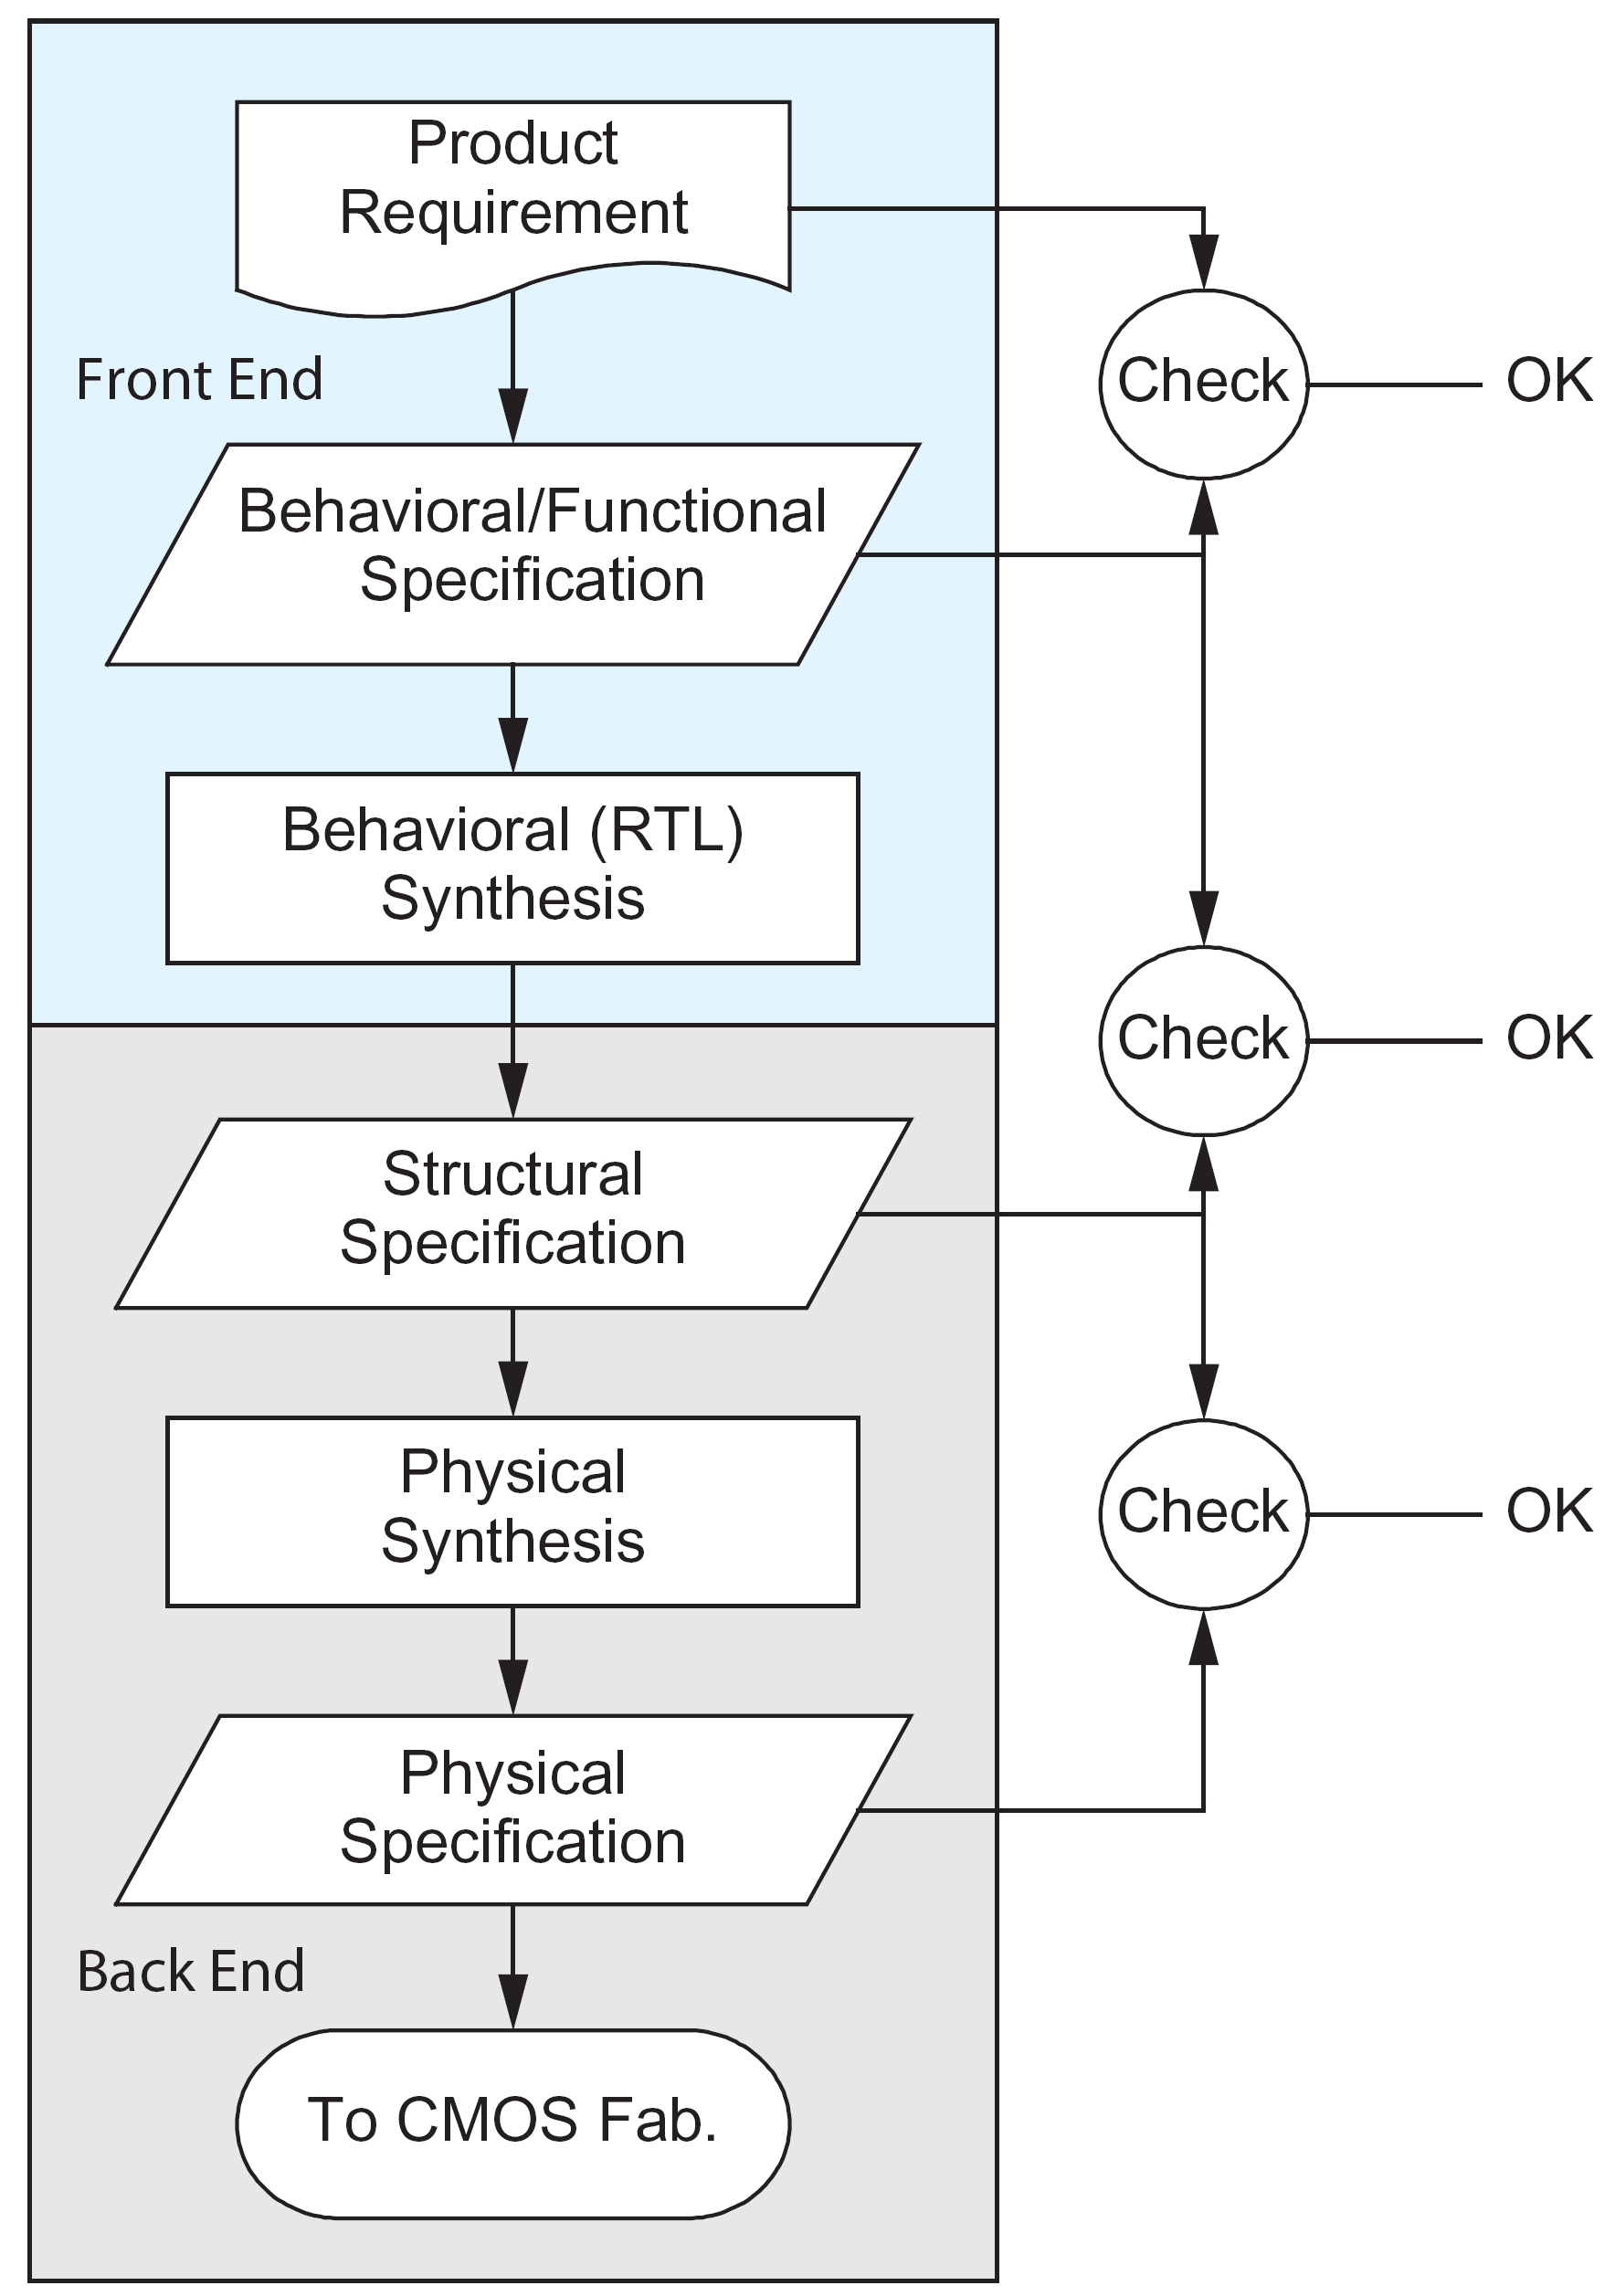
\includegraphics[width=0.25\textwidth]{fluxovlsi.png}
	\caption{Fluxo de projeto VLSI.}
	\label{fig:CMOS2010}
\end{figure}

No desenvolvimento do circuito, várias etapas são seguidas. Inicialmente, realiza-se a simulação comportamental para assegurar que o circuito descrito em VHDL cumpre os requisitos esperados, utilizando um \textit{testbench} em VHDL e a ferramenta Cadence NCLaunch. Posteriormente, ocorre a síntese lógica a partir do modelo comportamental, empregando a ferramenta Genus para gerar um modelo RTL com células padrão de uma tecnologia específica, levando em conta restrições de área, frequência e consumo de energia. Essa síntese resulta em dois arquivos: um em Verilog, contendo componentes e conexões, e outro com informações de atraso no formato SDF. A simulação pós-síntese é então executada para validar o netlist gerado, utilizando o mesmo \textit{testbench} da simulação comportamental. Na etapa de PAR, o layout é desenvolvido posicionando as células e estabelecendo as conexões entre elas, com o uso da ferramenta Innovus. Finalmente, na simulação pós-PAR, o circuito é avaliado considerando as resistências e capacitâncias parasitas. Cada etapa é crucial para assegurar o funcionamento correto do circuito.

